% Source: graduate-coursework/Sp26/CSCE763/Course_Assignments/Project/project_proposal.tex
% Description: RT-DETR transformer-based detector. End-to-end detection without NMS post-processing via learned object queries and cross-attention decoding.

\documentclass[border=4pt]{standalone}
\usepackage{amsmath}
\usepackage{amssymb}
\usepackage{graphicx}
\usepackage{tikz}
\usepackage{xcolor}
\usetikzlibrary{positioning, arrows.meta, calc, fit, backgrounds, decorations.pathreplacing}

\definecolor{USC_Garnet}{HTML}{73000A}
\definecolor{USC_Black10}{HTML}{ECECEC}
\definecolor{USC_Black70}{HTML}{5C5C5C}
\definecolor{USC_Congaree}{HTML}{1F414D}

\begin{document}
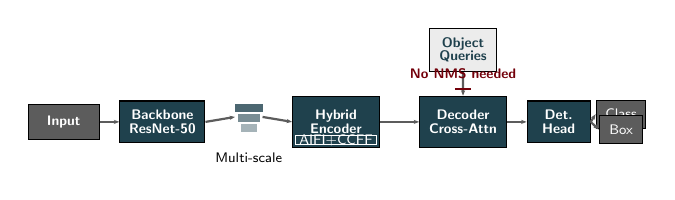
\begin{tikzpicture}[
  scale=0.7, every node/.style={font=\sffamily\tiny},
  block/.style={draw, fill=USC_Congaree, text=white, minimum height=0.45cm,
    minimum width=0.85cm, font=\sffamily\tiny\bfseries, align=center},
  nblock/.style={draw, fill=USC_Black70, text=white, minimum height=0.45cm,
    minimum width=0.85cm, font=\sffamily\tiny\bfseries, align=center},
  bgblock/.style={draw, fill=USC_Black10, minimum height=0.45cm,
    minimum width=0.85cm, font=\sffamily\tiny\bfseries, align=center,
    text=USC_Congaree},
  arr/.style={-{Stealth[length=2pt]}, thick, USC_Black70}
]
  % Input
  \node[nblock, minimum width=0.9cm] (inp) {Input};

  % Backbone
  \node[block, right=0.25cm of inp, minimum width=1.0cm] (back) {Backbone\\[-1pt]ResNet-50};

  % Multi-scale features (three stacked rectangles)
  \coordinate[right=0.55cm of back] (msc);
  \fill[USC_Congaree!80] ([yshift=0.18cm, xshift=-0.25cm]msc) rectangle ++(0.5cm,0.14cm);
  \fill[USC_Congaree!60] ([yshift=0.0cm, xshift=-0.2cm]msc) rectangle ++(0.4cm,0.14cm);
  \fill[USC_Congaree!40] ([yshift=-0.18cm, xshift=-0.15cm]msc) rectangle ++(0.3cm,0.14cm);
  \node[font=\sffamily\tiny, anchor=north] at ([yshift=-0.38cm]msc) {Multi-scale};

  % Hybrid Encoder
  \node[block, right=0.55cm of msc, minimum width=1.1cm, minimum height=0.65cm] (enc) {Hybrid\\[-1pt]Encoder};
  % Self-attention label inside encoder
  \draw[white, thin] ([yshift=0.06cm, xshift=0.06cm]enc.south west)
    rectangle ([yshift=0.22cm, xshift=-0.06cm]enc.south east);
  \node[white, font=\sffamily\tiny] at ([yshift=0.14cm]enc.south) {AIFI+CCFF};

  % Transformer Decoder
  \node[block, right=0.5cm of enc, minimum width=1.1cm, minimum height=0.65cm] (dec) {Decoder\\[-1pt]Cross-Attn};

  % Object Queries (parallel input from above)
  \node[bgblock, above=0.3cm of dec, minimum width=0.85cm] (oq) {Object\\[-1pt]Queries};

  % Detection Head
  \node[block, right=0.25cm of dec, minimum width=0.8cm] (head) {Det.\\[-1pt]Head};

  % Outputs (class + box)
  \node[nblock, minimum width=0.55cm, minimum height=0.22cm,
    font=\sffamily\tiny] (cls) at ([yshift=0.14cm, xshift=0.55cm]head.east) {Class};
  \node[nblock, minimum width=0.55cm, minimum height=0.22cm,
    font=\sffamily\tiny] (box) at ([yshift=-0.14cm, xshift=0.55cm]head.east) {Box};

  % Arrows
  \draw[arr] (inp) -- (back);
  \draw[arr] (back.east) -- ([xshift=-0.25cm, yshift=0.09cm]msc);
  \draw[arr] ([xshift=0.25cm, yshift=0.09cm]msc) -- (enc.west);
  \draw[arr] (enc) -- (dec);
  \draw[arr] (oq.south) -- (dec.north);
  \draw[arr] (dec) -- (head);
  \draw[arr] (head.east) -- (cls.west);
  \draw[arr] (head.east) -- (box.west);

  % "No NMS" annotation
  \draw[USC_Garnet, thick] ([yshift=0.12cm, xshift=-0.15cm]dec.north) --
    ([yshift=0.12cm, xshift=0.15cm]dec.north);
  \node[USC_Garnet, font=\sffamily\tiny\bfseries, anchor=south]
    at ([yshift=0.14cm]dec.north) {No NMS needed};
\end{tikzpicture}
\end{document}
